\mode*

\section{Fel och felhantering}

\subsection{Särfall}

\begin{frame}[fragile]
  \begin{example}
    \begin{lstlisting}
>>> int("a")
Traceback (most recent call last):
  File "<stdin>", line 1, in <module>
ValueError: invalid literal for int() with base 10: 'a'
>>> 
    \end{lstlisting}
  \end{example}
\end{frame}

\begin{frame}[fragile]
  \begin{example}
    \begin{lstlisting}
>>> 5/0
Traceback (most recent call last):
  File "<stdin>", line 1, in <module>
ZeroDivisionError: division by zero
>>> 
    \end{lstlisting}
  \end{example}
\end{frame}

\begin{frame}[fragile]
  \begin{example}
    \begin{lstlisting}
>>> prynt(3)
Traceback (most recent call last):
  File "<stdin>", line 1, in <module>
NameError: name 'prynt' is not defined
>>> 
    \end{lstlisting}
  \end{example}
\end{frame}

\subsection{Felhantering: att fånga särfall}

\begin{frame}
  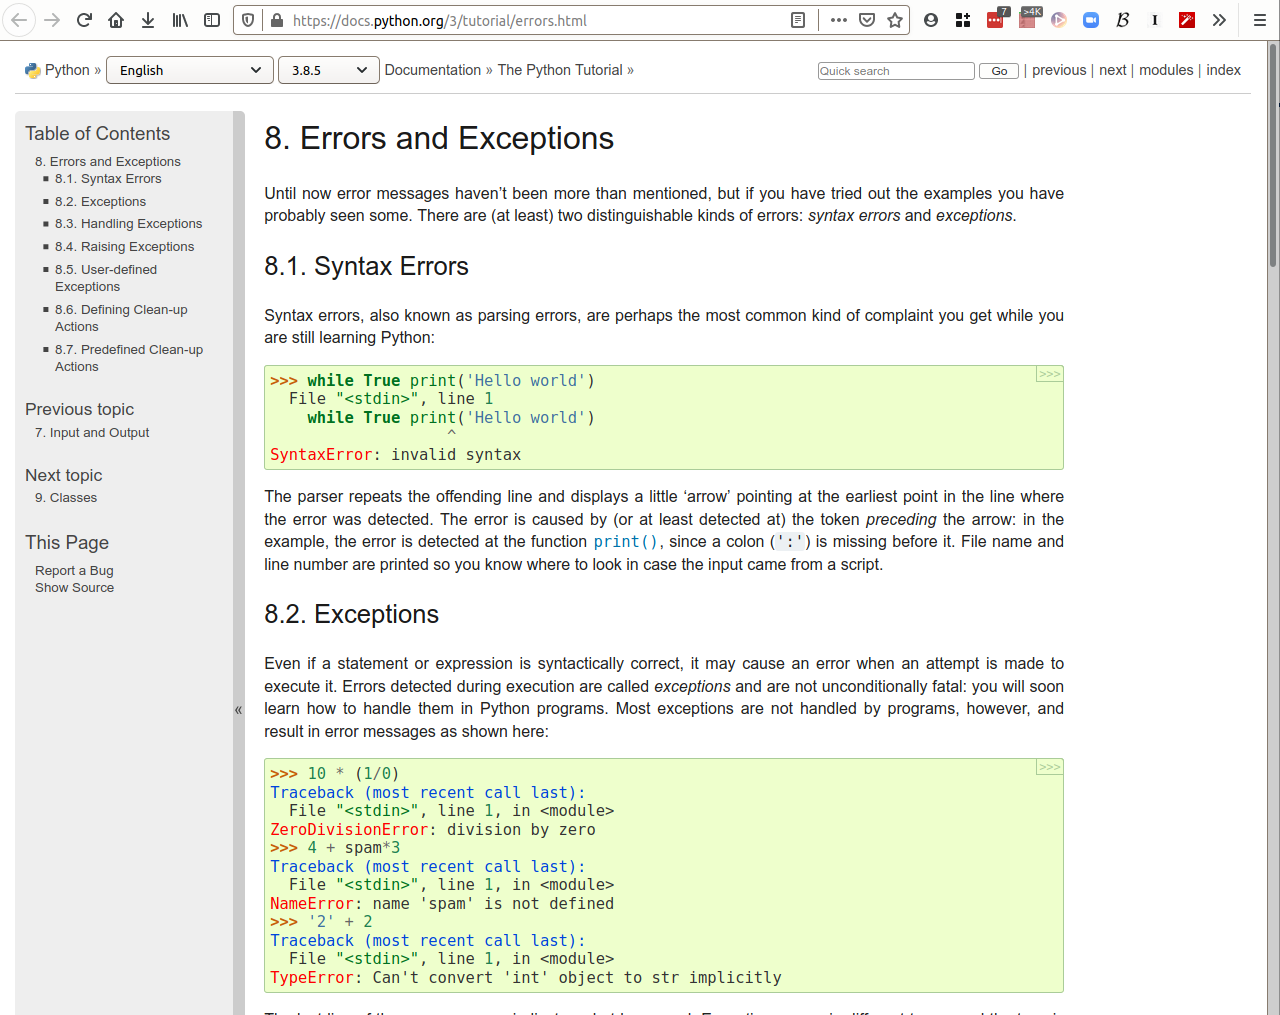
\includegraphics[width=\columnwidth]{figs/docs-except.png}
\end{frame}

\begin{frame}[fragile]
  \begin{example}[Fånga särfall: valuerr.py]
    \lstinputlisting{examples/valuerr.py}
  \end{example}

  \pause

  \begin{example}
    \begin{lstlisting}[language={}]
$ python3 valuerr.py
We caught this: invalid literal for int() with base 10: 'a'
    \end{lstlisting}
  \end{example}
\end{frame}

\begin{frame}[fragile]
  \begin{lstlisting}
try:
  # error
except Exception as err:
  print("Catch all errors!")
  \end{lstlisting}
  \begin{remark}
    \begin{itemize}
    \item \lstinline{except Exception as err} fångar \emph{allt}!
  \end{itemize}
  \end{remark}
\end{frame}

\begin{frame}[fragile]
  \begin{example}[manyerr.py]
    \lstinputlisting{examples/manyerr.py}
  \end{example}
\end{frame}

